\documentclass{cs202}

% =============================================
% Part 0 信息
% =============================================

\mathsetup{
  % 学生姓名
  student = {某同学},
  % 学号
  student-id = {2022****},
  % 院系
  institution = {数理学院数学系},
  % 专业年级
  discipline = {信息与计算科学专业 2022 级},
  % 日期
  date = {\today},
}

\begin{document}

% =============================================
% Part 1  封面
% =============================================

\makecover

% =============================================
% Part 2 主文档
% =============================================

\section{拴牛鼻的绳子}

农夫有一个长满草的半径为10米的圆形牛栏,他要将一头牛栓在栏桩上,但只让牛吃到一半草,问栓牛鼻的绳子应为多长?

\subsection{题目分析与思路}

\begin{figure}[H]  
    \centering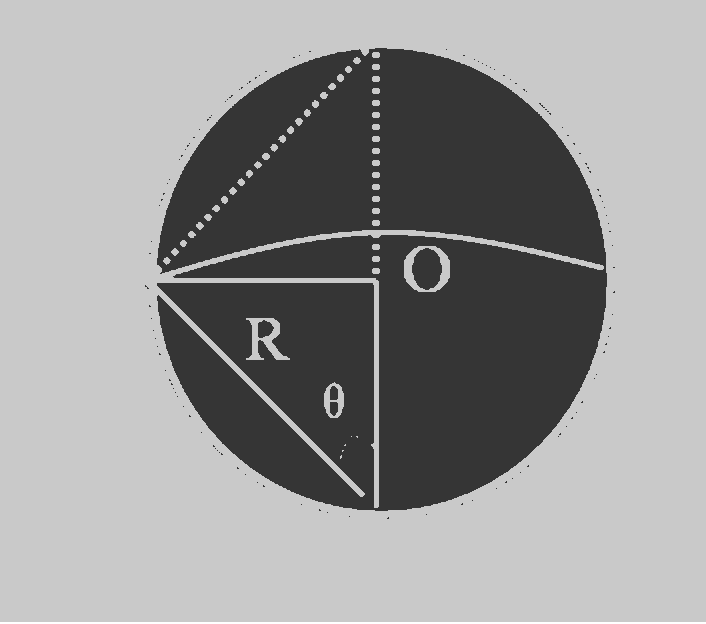
\includegraphics[width=0.3\linewidth]{01.png}  
    \caption{圆形牛栏示例}     
    \label{img01}   
\end{figure}
    
如图\ref*{img01}所示,设$A$为栓桩,绳$AB$长为$R$。
半径$OA=OB=r=10$,$\angle OAB=\theta$,那么$R=2r\cos\theta$。

由只让牛吃到一半的草,可得:
\begin{equation}
    \mbox{扇形}BAC\mbox{面积} + 2\mbox{冠形}ADB\mbox{面积} = \frac{1}{2}\pi r^2
\end{equation}
即
\[
    S_{\overset{\frown}{BAC}} + 2\times(S_{\overset{\frown}{BOA}} - S_{\Delta BOA}) = \frac{1}{2}\pi r
\]

\begin{equation*}
    \begin{split}
        \frac{2\theta}{2\pi}\pi R^2 + 2(\frac{\pi - 2\theta}{2\pi} - \frac{1}{2}Rr\sin\theta) = \frac{1}{2}\pi r^2 \\
        \Rightarrow \theta R^2 + 2(\frac{\pi - 2\theta}{2\pi} - \frac{1}{2}Rr\sin\theta) = \frac{1}{2}\pi r^2 \\
        \Rightarrow 4\theta\cos^2\theta + \pi - 2\theta - 2\cos\theta\sin\theta = \frac{1}{2}\pi
    \end{split}
\end{equation*}
从而得到关系式
\begin{equation}
    2\theta\cos^2\theta + \frac{\pi}{2} - \cos\theta\sin\theta - \frac{\pi}{4} - \theta = 0 \label{equation:1}
\end{equation}
或
\begin{equation}
    \theta = 2\theta\cos^2\theta + \frac{\pi}{2} - \cos\theta\sin\theta - \frac{\pi}{4}
\end{equation}
于是问题求解转化为一个关于$\theta$的非线性方程。

求解这个方程的根$\theta$的值,进而由关系式$R=2r\cos\theta$得到绳长。
\subsection{数值计算方法}

这里,采用不动点迭代法求解方程的根。(注,也可以采用其他求根方法)

设方程$f(\theta)=2\theta\cos^2\theta + \frac{\pi}{2} - \cos\theta\sin\theta - \frac{\pi}{4} - \theta = 0$的不动点迭代格式为
\begin{equation}
    \theta_{k+1}=\phi(\theta_k)=2\theta_k\cos^2\theta_k+\frac{\pi}{2}-\cos\theta_k\sin\theta_k-\frac{\pi}{4} \quad (k=0,1,2,\cdots)
\end{equation}

采用Python编写程序,取$\theta_0=0$,当迭代满足$|\theta_{k+1}-\theta_k|<0.00001$时,$\theta_{k+1}$为根的数值解,带入$R=2r\cos\theta$,得到$R$的值。

\subsection{Python代码}

\inputminted[
    frame=lines,
    framesep=2mm,
    baselinestretch=1.2,
    fontsize=\small,
    linenos
]{python}{code/lab01.py}

\subsection{结果分析}

方程\eqref{equation:1}的根为$\theta=0.9529$,绳长为$R=11.5872$。
所以农夫在长满草的半径10米的圆形牛栏,将一头牛栓在栏桩上,但只让牛吃到一半草,栓牛鼻的绳长应为11.5872米。

\section{机床加工零件的外形}

下表给出的$x, y$数据位于机翼断面的下轮廓线上,假设需要得到$x$坐标每改变0.1时$y$的坐标,试分段线性插值计算所需的数据,画出曲线,并分析结果。

\begin{center}
    \begin{tabular}{ccccccccccc}
        \toprule  %添加表格头部粗线
        x & 0 & 3   & 5   & 7   & 9   & 11  & 19  & 13  & 14  & 15  \\ 
        \midrule  %添加表格中横线
        y & 0 & 1.2 & 1.7 & 2.0 & 2.1 & 2.0 & 1.8 & 1.2 & 1.0 & 1.6 \\ 
        \bottomrule %添加表格底部粗线
    \end{tabular}
\end{center}


\subsection{数值计算方法}

分段线性插值公式:
\begin{equation}
    S_i(x)=y_{i-1}\frac{x-x_i}{x_{i-1}-x_i}+y_i\frac{x-x_{i-1}}{x_i-x_{i-1}}
\end{equation}

事实上,分段线性插值函数是在两个节点构成的区间上实行$n-1$的拉格朗日插值得到的线性函数。
用拉格朗日插值和分段线性插值计算所需的数据,并利用Python编写程序,分别得到坐标$x$每改变0.1时的对应$y$坐标,画出曲线,进行分析。

\subsection{Python代码}
\inputminted[
    frame=lines,
    framesep=2mm,
    baselinestretch=1.2,
    fontsize=\small,
    linenos
]{python}{code/lab02.py}

\subsection{结果分析}

采用分段线性插值计算所得结果如图\ref*{img02}所示,其中图像经过一定的后处理。
从图中可以看出分段线性插值结果与原始数据吻合较好。

\begin{figure}[H]  
    \centering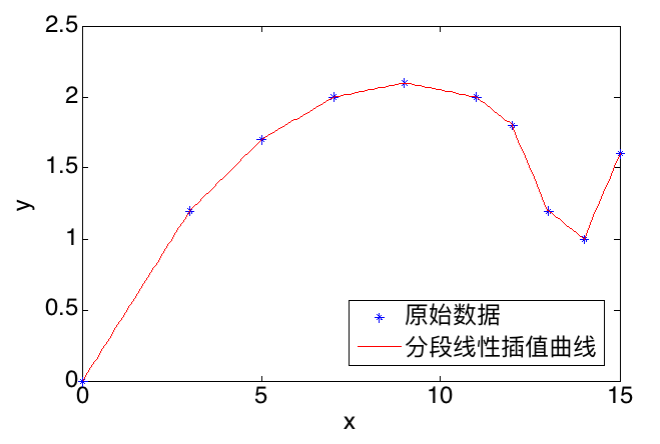
\includegraphics[width=0.8\linewidth]{02.png}  
    \caption{分段线性插值结果与原始数据的比较}     
    \label{img02}   
\end{figure}

% =============================================
% Part 3  读后感
% =============================================

\section{必读材料读后感}

% 请删除\todo部分,并开始编写你的读后感
\todo[inline,color=blue!20]{请于课程最后一次提交报告之前在此处填写不少于500字的读后感}

% =============================================
% Part 4 课程建议
% =============================================

\section{课程反馈和建议}

% 请删除\todo部分,并开始编写你的课程建议
\todo[inline,color=green!40]{由于本课程为全新版课程,需要了解同学们真实的上课反应,以便于对课程内容进行适当更新。
请基于你的上课感受,给出你对课程的反馈和建议。}

\end{document}
